\documentclass[tikz,border=5mm]{standalone}
\usepackage{pgfplots}
\pgfplotsset{compat=1.18}

\begin{document}

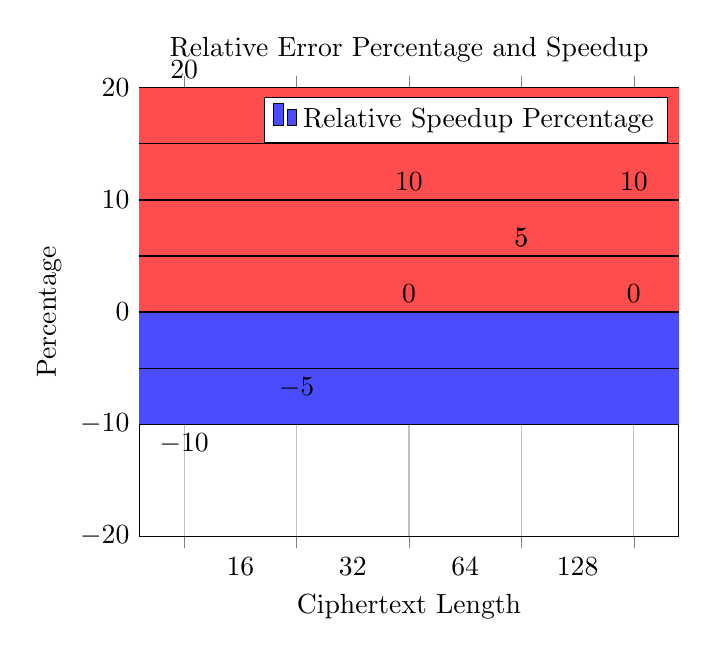
\begin{tikzpicture}
    \begin{axis}[
        title={Relative Error Percentage and Speedup},
        xlabel={Ciphertext Length},
        ylabel={Percentage},
        ymin=-20,
        ymax=20,
        ybar interval=20pt,
        bar width=30pt,
        symbolic x coords={16, 32, 64, 128, 256},
        xtick=data,
        nodes near coords,
        nodes near coords align={vertical},
        ]
        
        % Relative Error Percentage Data
        \addplot[fill=blue!70] coordinates {(16,-10) (32,-5) (64,0) (128,5) (256,10)};
        \legend{Relative Error Percentage}
        
        % Relative Speedup Percentage Data
        \addplot[fill=red!70] coordinates {(16,20) (32,15) (64,10) (128,5) (256,0)};
        \legend{Relative Speedup Percentage}
        
    \end{axis}
\end{tikzpicture}

\end{document}